\documentclass[11pt, oneside]{article} 
\usepackage{geometry}
\geometry{letterpaper} 
\usepackage{graphicx}
	
\usepackage{amssymb}
\usepackage{amsmath}
\usepackage{parskip}
\usepackage{color}
\usepackage{hyperref}

\graphicspath{{/Users/telliott_admin/Tex/png/}}
% \begin{center} 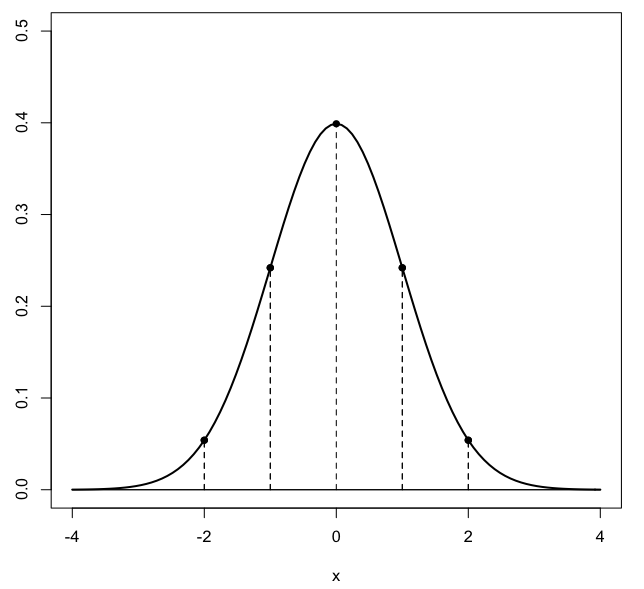
\includegraphics [scale=0.4] {gauss3.png} \end{center}

%break
\title{Trigonometric integrals}
\date{}

\begin{document}
\maketitle
\Large

\label{sec:Inverse_trig}

\subsection*{Inverse sine}
This is our first of the inverse trigonometric functions (there are only two really important ones).
\[ y = \sin^{-1} x \]
Read this as $y$ is the arc sine or inverse sine of $x$.  

More usefully,  we can say that $y$ is the angle whose sine is $x$.  This means the same thing, we have just solved the first equation for $x$:
\[ x = \sin y \]
Plot the angle as a function of its sine.
\begin{center} 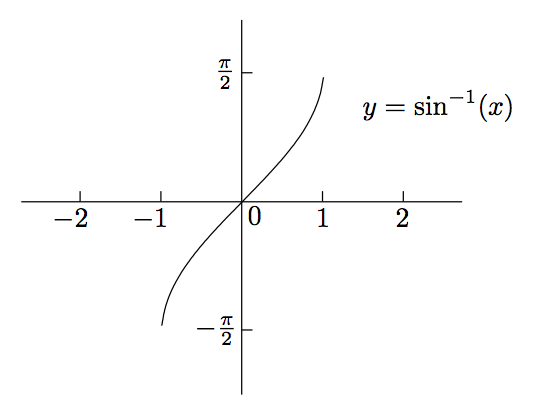
\includegraphics [scale=0.4] {arcsin.png} \end{center}
The graph is the same shape as the standard sine curve, but flipped and rotated 90 degrees.

We need to be careful about the interval on which we're working, since if we go too far we will duplicate values and thus, no longer have a \emph{function}.  You can see from the plot that the range of $y$ should be $[-\pi/2,\pi/2]$.

We can derive something useful from this with a trig substitution:
\begin{center} 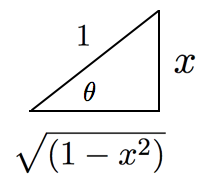
\includegraphics [scale=0.5] {trig1.png} \end{center}

Basic trigonometry says that if
\[ x = \sin \theta \]
\[ \theta = \sin^{-1} x \]
then
\[ \cos \theta = \sqrt{1 - x^2} \]
so differentiating
\[ \frac{dx}{d \theta} = \frac{d}{d \theta} \sin \theta = \cos \theta = \sqrt{1 - x^2} \]
Inverting
\[ \frac{d \theta}{dx} = \frac{1}{\sqrt{1 - x^2}} \]

Furthermore, integrating:
\[ \int \frac{1}{\sqrt{1 - x^2}} \ dx = \int d \theta = \theta \]
\[ = \sin^{-1} x \]
and
\[ \frac{d}{dx} \sin^{-1} x =  \frac{1}{\sqrt{1 - x^2}} \]
This integral arises in many problems.

Let's switch to using $t$ for $\theta$.  Another derivation is to say 
\[ x = \sin t \]
\[ dx = \cos t \ dt \]
so the integral is
\[ \int \frac{1}{\sqrt{1 - x^2}} \ dx = \int \frac{1}{\cos t}  \cos t \ dt = t \]

The complementary angles of a right triangle add up to $\pi/2$, thus
\[ \sin^{-1} t + \cos^{-1} t = \pi/2 \]

Here's a picture of the two functions together.  It is not hard to believe they add up to a constant.
\begin{center} 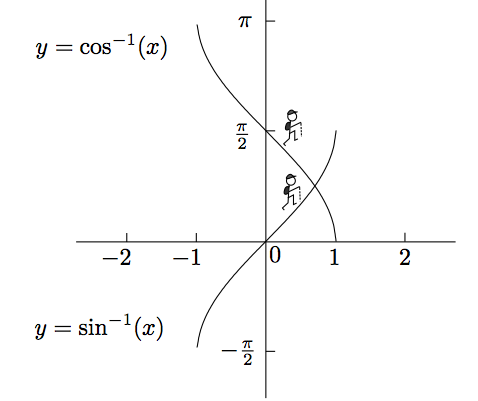
\includegraphics [scale=0.4] {arcsincos.png} \end{center}

We find the inverse cosine easily by differentiating:
\[ \sin^{-1} t + \cos^{-1} t = \pi/2 \]
\[ \frac{d}{dt} \sin^{-1} t + \frac{d}{dt}  \cos^{-1} t = 0 \]
\[ \frac{d}{dt} \sin^{-1} t = - \frac{d}{dt}  \cos^{-1} t \]
where we had
\[ \frac{d}{dt} \sin^{-1} t = \frac{1}{\sqrt{1 - x^2}} \]
The inverse cosine isn't seen that much because its the very same problem as the inverse sine.  

\subsection*{inverse tangent}
However, the inverse tangent is important.  Let
\[ x = \tan t \]
\[ t = \tan^{-1} x \]

Differentiating the first equation
\[ \frac{dx}{dt} = \sec^2 t \]
If you haven't seen this before, try using the quotient rule on $\sin t / \cos t$.
Inverting
\[ \frac{dt}{dx} = \cos^2 t \]

Basic trigonometry will show that if
\[ x = \tan t \]
then the hypotenuse must be $\sqrt{1 + x^2}$ so
\[ \cos t = \frac{1}{\sqrt{1 + x^2}} \]
and then
\[ \frac{dt}{dx} = \cos^2 t = \frac{1}{1 + x^2} \]

Integrate
\[ \int dt = \int \frac{1}{1 + x^2} \ dx  \]
\[ t = \int \frac{1}{1 + x^2} \ dx  \]
But $t = \tan^{-1} x$ so
\[ \tan^{-1} x = \int \frac{1}{1 + x^2} \ dx  \]

We will show elsewhere that
\[ (1 + x^2) \cdot (1 - x^2 + x^4 - x^6 + \dots) = 1 \]
You can check by multiplying it out.  

Rearrange and integrate
\[    \int \frac{1}{1+x^2} \ dx =  \int 1 - x^2 + x^4 - x^6 + \dots \ dx \]
\[ = x - \frac{x^3}{3} + \frac{x^5}{5} - \frac{x^7}{7} + \dots \]
Combining with what's above
\[ \tan^{-1} x = x - \frac{x^3}{3} + \frac{x^5}{5} - \frac{x^7}{7} + \dots \]
The angle whose tangent is $1$ is $\pi/4$ so
\[ \frac{\pi}{4} = 1 - \frac{1}{3} + \frac{1}{5} - \frac{1}{7} + \dots \]
This is the first of a number of series that yield $\pi$.

\end{document}